\documentclass[conference,10pt]{IEEEtran}

\usepackage{cite}
\usepackage{amsmath}
\usepackage{newtxmath}
\usepackage{graphicx}
\graphicspath{{../src/figs/}}
\usepackage{booktabs}
\usepackage{algorithm}
\usepackage{algpseudocode}
\usepackage{url}
\usepackage{subcaption}
\usepackage{stfloats}
\makeatletter\newcommand{\inputtable}[1]{\@@input #1 }\makeatother

% =============================================================================
% HOW TO USE THIS FILE
% -----------------------------------------------------------------------------
% Every section below has a heading and comments only. Lines starting with
%   %  -  are points the section must make.
%   %  >  are explanations of a concept you need to understand first.
%   %  [fig] / [tab]  are ready-made figure and table blocks: uncomment to use.
% Numbers quoted here come from src/results/ and PLAN.md (log, 2026-10-13).
% Check a number against its file before it goes into the text.
%
% Build:  latexmk -pdf -outdir=aux 26989395RW741assignment4.tex
% Submit: aux/26989395RW741assignment4.pdf, renamed to sit in report/.
%
% Marks (150): abstract 4, introduction 8, background 24, implementation 8,
% empirical process 18, results and discussion 48, conclusions 4,
% references 4, linguistic quality 32. Results and discussion is a third of
% the mark: give it about four of the ten pages.
%
% Brief requirements that are easy to miss:
%  - justify the CHOICE of ensemble method (similar or dissimilar to the
%    assignment 2 models, with an argument);
%  - justify the tuning: questions set out before evaluation;
%  - background AND implementation detail for the assignment 2 models
%    (k-NN and the tree), not only for the forest;
%  - justify any data transformation;
%  - student number in the title block, NO name, surname or other identifying
%    information; link to the Git repository.
%
% Marker feedback on assignment 2 to answer (see PLAN.md section 3):
%  - figure font the same as the paper (done in plotstyle.py);
%  - a curve for every tuned parameter;
%  - every number discussed must be in a table or figure;
%  - no extreme or edge selected values without comment;
%  - cite the original papers;
%  - formal register: no "wins", "beats", "gap"; few bulleted lists;
%  - ten pages or fewer.
% =============================================================================

\begin{document}

\title{A Random Forest for Network Intrusion Classification on UNSW-NB15}
% - Assignment 2 used a two-part title ("Rooted in the Neighbourhood: ...").
%   A matching pattern keeps the series consistent.
% - The subtitle names the method and the task: random forest, network
%   intrusion detection / UNSW-NB15.

\author{
  \IEEEauthorblockN{26989395}
  \IEEEauthorblockA{RW741}
}
% - Brief: student number required; name, surname and similar identifying
%   information NOT allowed. Assignment 3 carried "A. Cottrell" and an email
%   address; both are left out here on purpose.
% - Confirm the module code (RW741) before submission; the file name uses it.

\maketitle

\begin{abstract}
% - One paragraph, about 150 to 200 words, no citations, no lists.
% - In order (style guide, section 6): what the data is, what method was used,
%   the headline number, one honest caveat.
% - Data: UNSW-NB15 network traffic records, ten classes, heavily imbalanced,
%   46.5% duplicate records, 15.7% in groups with conflicting labels.
% - Method: a random forest implemented from scratch, tuned by five research
%   questions on five-fold cross-validation, compared with the assignment 2
%   classification tree and k-NN classifier.
% - Headline: macro F1 0.6102 against 0.5860 (tree) and 0.5010 (k-NN); the
%   forest was higher on all five folds against both (Holm-corrected paired
%   t-tests, p = 0.00015 and 0.00005).
% - Insight: feature subsampling helped and the bootstrap did not; the best
%   number of features per split (14) was more than twice the usual square
%   root; no imbalance treatment raised macro F1.
% - Caveat: the classes with conflicting duplicates (Backdoor, DoS, Analysis)
%   stay at F1 0.18 to 0.33, because no classifier can separate records with
%   identical features.

The UNSW-NB15 dataset holds 257,673 network flow records in ten classes of
very different sizes. Almost half of the records are duplicates, and about
one in six sits in a group of identical records with conflicting classes. A
random forest was implemented and tuned on five-fold cross-validation
through five research questions set before the experiments. It
was compared with the classification tree and the k-nearest neighbours
classifier of assignment 2. The selected forest scores 0.6102 on the
macro-averaged $F_1$ score, against 0.5860 for the tree and 0.5010 for the
k-nearest neighbours classifier, and scores higher than both on all five folds.
The best forest draws more than twice the usual number of features at each
split and uses no bootstrap. None of the four imbalance treatments
raised the score. Backdoor, Analysis and DoS, whose records mostly sit in
conflicting groups, remain the weakest classes, because
no classifier can separate records with identical features.
\end{abstract}

\begin{IEEEkeywords}
% - Four to six terms: random forest, ensemble learning, intrusion detection,
%   class imbalance, UNSW-NB15.
Random forest, ensemble learning, intrusion detection, class imbalance,
UNSW-NB15
\end{IEEEkeywords}

% =============================================================================
\section{Introduction}
\label{sec:introduction}
% Worth 8. About three quarters of a column. No subsections.
%
% - Problem: intrusion detection as multi-class classification of network
%   records; why misclassifying rare attack classes matters.
% - What assignment 2 found and why it motivates this report: the tree
%   (0.5872 macro F1 in assignment 2) beat k-NN (0.5010) but showed high
%   variance (training 0.78 against validation 0.59), and three features
%   carried about 65% of its importance. Variance is the problem a random
%   forest is designed to reduce.
% - The choice of ensemble, stated as an argument (the brief asks for one):
%   a random forest is an ensemble of the assignment 2 tree, so the
%   comparison isolates the effect of combining trees. A dissimilar method
%   (boosting, a stacked model) would change two things at once.
% - The five research questions, one sentence each, stated as questions:
%   number of trees; sources of randomness; tree complexity; imbalance
%   treatment; choice of performance measure.
% - Contributions in one or two sentences: own implementation of the tree,
%   forest, SMOTE and Tomek links; a protocol fixed before the results.
% - Last paragraph: outline of the remaining sections, one sentence each
%   (style guide: the Introduction ends with the section outline).

An intrusion detection system decides which of the exchanges crossing a
network are attacks. In assignment 2 this decision was treated as a
classification problem on the UNSW-NB15 dataset~\cite{moustafa2015unsw}. Two models were compared there. The
classification tree scored 0.5872 on the macro-averaged $F_1$ score against
0.5010 for the k-nearest neighbours classifier, but it also showed the signs
of high variance. An unconstrained tree scored 0.7806 on its training records
and 0.5791 on the validation records, and three features carried roughly two
thirds of its decisions.

A random forest is designed to reduce the variance of a single
tree~\cite{breiman2001random}. It grows many trees, each on a random sample
of the records and each choosing its splits from a random subset of the
features, and classifies a record by the majority vote of the trees.
Averaging over trees that make different errors cancels part of the variance
of a single tree, and restricting the features at each split stops every tree
from being built around the same three features. The random forest was chosen
over other ensemble methods because it is an ensemble of the same
classification tree. The comparison with assignment 2 therefore changes one
thing, the combining of trees, where boosting or a stacked model would change
the underlying model as well.

The tree, the forest and the resampling methods were implemented for this
report. The forest was tuned and evaluated on the same five cross-validation
folds as assignment 2, so the forest is compared fold by fold with both
earlier models. The experiments answer five research questions, set out in
Section~\ref{subsec:emp_questions}. They concern the number of trees, the
two sources of randomness, the depth and leaf size of the trees, the
treatment of the class imbalance and the choice of performance measure.

The forest scores 0.6102 on the macro-averaged $F_1$ score, against 0.5860
for the tree, retuned for this report, and 0.5010 for the k-nearest
neighbours classifier, and scores higher than both on every fold.  With the usual six
features per split the forest scored below the single tree, and the random
sample of records lowered the score at every number of features below 42.
The classes whose records share their features with records of other classes
remain the weakest for every model, as they were in assignment 2.

Section~\ref{sec:background} gives the background on the dataset, the
models, the treatment of imbalance and the measures.
Section~\ref{sec:implementation} describes the implementation and its
verification, Section~\ref{sec:empirical} the research questions and the
protocol, and Section~\ref{sec:results} the results and their discussion.
Section~\ref{sec:conclusion} concludes.

% =============================================================================
\section{Background}
\label{sec:background}
% Worth 24, the second largest share. About two pages.
% - Define every concept the later sections use, and nothing they do not.
% - Cite the ORIGINAL paper for each method (marker feedback).
% - One opening sentence saying what the section covers.

This section describes the dataset and the two models of assignment 2, then
defines the ensemble methods, the treatments of class imbalance, the
performance measures and the statistical procedures used in the later
sections.

\subsection{Network intrusion detection and the UNSW-NB15 dataset}
\label{subsec:bg_dataset}
% - Intrusion detection systems; misuse against anomaly detection; why
%   machine learning (cite buczak2016survey).
% - UNSW-NB15: origin, synthetic traffic generated with IXIA PerfectStorm
%   (cite moustafa2015unsw); the ten classes.
% - Keep the data-quality findings for the Implementation section; here only
%   what the dataset is.

A network flow record summarises one exchange between two hosts. The record holds counts and timings, such as the bytes sent each way and the
duration, rather than the contents of the exchange. An intrusion detection system reads such records
and decides which of them represent an attack. Treating this decision as a classification problem is the usual
approach~\cite{buczak2016survey}. Each record is an instance, the counts and timings are the
descriptive features, and the class is the kind of attack the record
represents, or ordinary traffic if it represents none.

The UNSW-NB15 dataset was created at the Cyber Range Lab of UNSW
Canberra~\cite{moustafa2015unsw}. The IXIA PerfectStorm tool generated a mix
of real ordinary traffic and synthetic attacks, and the captured traffic was
summarised into flow records. The 257,673 records used here are the
published training and testing sets combined. Each record has 42
descriptive features and one of ten classes. Three of the features are
nominal: the protocol, the service and the connection state of a flow. The
classes are Normal and nine attack categories: Generic, Exploits, Fuzzers,
DoS, Reconnaissance, Analysis, Backdoor, Shellcode and Worms. The class
sizes range from 93,000 Normal records to 174 Worms records, a ratio of
about 534 to one.



\subsection{The k-nearest neighbours classifier}
\label{subsec:bg_knn}
% - Required by the brief: background for the assignment 2 models.
% - Classification by majority class of the k nearest training records
%   (cite cover1967nearest).
% - Distance measures: Euclidean, Manhattan; why Manhattan can be preferred
%   in many dimensions (cite aggarwal2001surprising).
% - Sensitivity to feature scale and to irrelevant features; cost at
%   prediction time (every query scans the training set).
% - Can be shortened from the assignment 2 report.

The k-nearest neighbours classifier stores the training records and does
nothing else until it is asked to classify~\cite{cover1967nearest}. To
classify a record, it measures the distance from that record to every stored
record, takes the $k$ closest, and assigns the class that most of them hold.


Two choices define the classifier. The first is $k$. A small $k$ follows the fine detail of the boundary between classes but lets
a single misleading record decide, while a large $k$ steadies the answer and
blurs any narrow boundary. The second is the distance itself. The Manhattan distance, the sum of the absolute differences, is often
preferred to the Euclidean distance when there are many
features~\cite{aggarwal2001surprising}.

The distance sums a contribution from every feature, so a feature measured
in large units contributes more than a feature measured in small ones,
whatever either feature means. Features must therefore be brought onto a
comparable scale before the distance is meaningful. Fitting costs nothing, and every prediction costs a pass over the stored
records.

\subsection{Classification trees}
\label{subsec:bg_tree}
% - Recursive partitioning; impurity measures, Gini and entropy, with their
%   formulas (cite breiman1984cart, quinlan1986induction).
% - Information gain as the decrease in weighted impurity; greedy split
%   choice; numeric thresholds and nominal splits.
% - Gini and entropy rarely choose different splits (cite
%   raileanu2004theoretical); the tree grid found them within noise.
% - Stopping and complexity control: maximum depth, minimum leaf size.
% - High variance: small changes in the data change the tree. This is the
%   bridge to ensembles, so state it plainly.
% - Impurity-based feature importance: total weighted impurity decrease per
%   feature, normalised. Its known bias towards features with many split
%   points (cite strobl2007bias) matters for the importance discussion.

A classification tree splits the training records into two groups by testing
one feature, then splits each group again, and continues until a stopping
rule applies~\cite{breiman1984cart}. Each leaf holds the records that
reached it, and a new record is classified by following the tests down to a
leaf and taking the majority class there.

The test at each node is chosen to make the resulting groups as pure as
possible, where a pure group holds records of one class only. For a group
$S$ in which a proportion $p_c$ of the records belong to class $c$, the Gini
index and the entropy are
\begin{equation}
  G(S) = 1 - \sum_{c} p_c^2, \qquad
  H(S) = -\sum_{c} p_c \log_2 p_c .
\end{equation}
Both are zero for a pure group and largest when every class is equally
common. The Gini index comes from~\cite{breiman1984cart} and the entropy
from~\cite{quinlan1986induction}, and the two rarely choose different
splits~\cite{raileanu2004theoretical}. A split of $S$ into $S_L$ and $S_R$
is scored by the decrease in impurity it achieves, called the information
gain when the impurity is the entropy:
\begin{equation}
  \Delta I = I(S) - \frac{|S_L|}{|S|} I(S_L) - \frac{|S_R|}{|S|} I(S_R),
\end{equation}
where $I$ is either measure and $|S|$ is the number of records in $S$. The
tree takes the split with the largest decrease at each node and never
revisits it, so the search is greedy. 

On its own, a tree keeps splitting until every leaf is pure, which usually
means it has memorised the training records rather than learned anything
general. Growth is therefore constrained: a maximum depth limits the number of tests on the path from the root to a leaf, and a minimum leaf size stops a split that would leave
too few records behind.

Even when constrained, a tree has high variance. A small change in the
training records can change the split chosen near the root, and every split
below it changes with it.  Ensembles of trees address this weakness.

A split depends only on the order of the values of a feature, so rescaling a
feature has no effect on the tree, unlike the k-nearest neighbours
classifier.

The importance of a feature is the total decrease in impurity of the splits
that test it, weighted by the number of records each split divides, and
divided by the total over all features so that the importances sum to one.
This measure favours features with many possible split points, because a
feature with more distinct values offers more chances to find a good split
by luck~\cite{strobl2007bias}.

\subsection{Ensemble learning}
\label{subsec:bg_ensemble}
% - Definition: combine several models into one prediction (cite
%   dietterich2000ensemble).
% - Why it works: the errors of the members must be partly independent.
%   Diversity is the key word.
% - Three families in one sentence each: bagging, boosting, stacking. Then
%   why this report takes the bagging family.
%
% > Bias and variance. A model's expected error splits into bias (systematic
%   error from a too-simple model), variance (how much the model changes with
%   the training sample) and irreducible noise. A deep tree has low bias and
%   high variance. Averaging many such trees leaves the bias about the same
%   and lowers the variance, which is why forests use deep trees.
% > The key formula (ESL, hastie2009elements, Eq. 15.1): for B identically
%   distributed models, each with variance sigma^2 and pairwise correlation
%   rho, the variance of their average is
%       rho * sigma^2 + (1 - rho) / B * sigma^2.
%   The second term vanishes as B grows; the first does not. More trees
%   therefore help only up to a point, and the only way to lower the
%   remaining variance is to lower rho, the correlation between the trees.
%   Everything a random forest adds to bagging is there to lower rho. Put
%   this formula in the report: Results Q1 and Q2 both lean on it.

An ensemble combines the predictions of several models into
one~\cite{dietterich2000ensemble}. For classification, the members are usually combined by a majority vote,
which helps only when they make different errors.  The members must therefore be diverse, meaning that their errors
are at least partly independent.

A deep tree has low bias and high variance: it can follow almost any
boundary, but follows a different one for every sample. Averaging many deep
trees lowers the variance and leaves the bias about the
same~\cite{hastie2009elements}.

The gain from averaging is limited by how alike the members are. Consider
$B$ models whose predictions each have variance $\sigma^2$, and let $\rho$
be the correlation between the predictions of any two of them. The variance
of their average is~\cite[Eq.~15.1]{hastie2009elements}
\begin{equation}
  \rho\sigma^2 + \frac{1-\rho}{B}\,\sigma^2 .
\end{equation}
The second term shrinks towards zero as $B$ grows, but the first does not
depend on $B$. Adding members therefore helps only up to a point, after
which the only way to lower the variance further is to lower $\rho$, the
correlation between the members.

Ensemble methods differ in how they make their members diverse. Bagging
trains each member on a different random sample of the records and gives
every vote the same weight. Boosting trains the members one after another, each giving more weight to
the records that the earlier members misclassified.
Stacking trains a second model to combine the predictions of several
different kinds of model. Bagging lowers the variance of its members, while
boosting mainly lowers their bias. This report therefore takes the bagging
family, because the weakness of the assignment 2 tree is its variance.
Everything that the random forest adds to bagging is there to lower $\rho$.

\subsection{Bagging and random forests}
\label{subsec:bg_rf}
% - Bagging: each tree on a bootstrap sample, majority vote (cite
%   breiman1996bagging).
% - Random subspace method: each tree on a random subset of features (cite
%   ho1998random).
% - Random forest: bootstrap plus a random subset of features at every split
%   (cite breiman2001random). Default features per split: square root of the
%   feature count for classification, about 6 of 42 here.
% - Majority vote against averaging class probabilities; this implementation
%   votes, as in Breiman's paper.
% - Extremely randomised trees (cite geurts2006extremely) drop the bootstrap
%   and rely on other randomness. Worth one sentence: the selected forest
%   also has no bootstrap, so it is not a standard random forest, and this
%   is the published precedent for that design.
% - Number of trees: more trees do not overfit, the score levels off (cite
%   breiman2001random, probst2018tune).
%
% > The bootstrap. A sample of n records drawn with replacement from n. Each
%   record is left out with probability (1 - 1/n)^n, about 1/e = 0.368, so
%   each tree sees about 63.2% of the distinct records, some several times.
%   Here 46.5% of records are duplicates, so a left-out record often still
%   has an identical copy in the sample. This is why the bootstrap adds less
%   diversity on this dataset than usual.
% > Features per split (often called mtry). Fewer features per split makes
%   the trees more different (lower rho) but each tree weaker (higher
%   sigma^2 and bias). The best value balances the two. With all features
%   and a bootstrap the forest is bagging; with all features and no
%   bootstrap every tree is the same tree.

Bagging, short for bootstrap aggregating, is the simplest method of the
family~\cite{breiman1996bagging}. Each tree is grown on a bootstrap sample,
which is a sample of $n$ records drawn with replacement from the $n$
training records. A record is missed by one draw with probability $1-1/n$,
and by the whole sample with probability $(1-1/n)^n$, which is about
$1/e \approx 0.368$ for large $n$. Each tree therefore sees about 63.2\% of
the distinct records, and about 26.4\% of the records appear two or more times. The trees are then
combined by a majority vote.

Bagging changes only the records that a tree sees. When a few features
separate the classes far better than the rest, every tree still splits on
those features near its root, so the trees stay alike and their correlation
$\rho$ stays high. The random subspace method instead grows each tree on a
random subset of the features~\cite{ho1998random}. The random forest
combines the two ideas~\cite{breiman2001random}. Each tree is grown on a
bootstrap sample, and at every node the split is chosen from a new random
subset of $m$ features rather than from all of them. The usual value of $m$
for classification is the square root of the number of features, which is
about six of the 42 features here. 

The number of features per split sets a trade-off. A small $m$ makes the
trees more different from one another, which lowers $\rho$. Each tree is
weaker, however, because the best feature for a split is often not among
those drawn, which raises the variance $\sigma^2$ of each tree and the bias.
A large $m$ gives strong but similar trees, and the best value lies between
the two and depends on the data. With all 42 features at every split the
forest becomes bagging. With all 42 features and no bootstrap, every tree is
grown on the same records with the same choices, so every tree is the same
tree.

The bootstrap is not the only source of diversity. Extremely randomised
trees drop the bootstrap and grow every tree on all of the records, relying
instead on random features and random thresholds at each
split~\cite{geurts2006extremely}. The forest selected in this report also has no bootstrap but keeps the best threshold
at each split, so its only source of diversity is the random set of 14
features drawn at each split.

Adding trees does not make a random forest overfit~\cite{breiman2001random}.
The score rises quickly over the first trees and then levels
off~\cite{probst2018tune}, so the number of trees trades computing time
against a shrinking gain.

\subsection{Learning from imbalanced classes}
\label{subsec:bg_imbalance}
% - The problem: a classifier that minimises errors favours the common
%   classes (cite he2009learning).
% - Class weighting: weight each record by the inverse frequency of its class.
% - Balanced random forest: each tree draws the same number of records from
%   every class (cite chen2004using).
% - SMOTE: synthetic minority records by interpolation between a record and
%   one of its k nearest same-class neighbours (cite chawla2002smote).
% - Tomek links: a pair of records from different classes that are each
%   other's nearest neighbour (cite tomek1976two). Removing them cleans the
%   class boundary. SMOTE followed by Tomek removal is the marker's
%   suggestion (cite batista2004study for the combination).
%
% > Why Tomek links matter here. Two records with identical features and
%   different labels are at distance zero, so each is the other's nearest
%   neighbour: they always form a Tomek link. Removing both records deletes
%   every conflicting duplicate group from the training data. The training
%   set then looks clean, but the validation fold still contains the
%   conflicts. This is the mechanism behind hypothesis 4, part two.

A classifier that minimises the number of errors favours the common classes,
because an error on a rare class costs no more than an error on a common one
and the common classes supply most of the records~\cite{he2009learning}.  Treatments of imbalance either change how much each record
counts, or change the records themselves.

Class weighting gives each record a weight equal to the inverse frequency of
its class, so that a rare class counts for as much in the impurity as a
common one. The balanced random forest changes the sample of each tree
instead~\cite{chen2004using}. Each tree draws the same number of records
from every class with replacement, usually as many as the smallest class
holds, so that every tree is grown on balanced data. 

Resampling methods change the training records before any model is grown.
SMOTE adds synthetic records to a rare class~\cite{chawla2002smote}. For
each new record, it picks a record of the class and one of its $k$ nearest
neighbours from the same class, and places the new record at a random point
on the line between the two. A nominal feature of the new record takes the
level held by most of the $k$ neighbours. The rare class is therefore
enlarged with records that resemble its own, rather than with exact copies,
which lead a tree to grow small regions around the copied records.

A Tomek link is a pair of records from different classes in which each record is the nearest neighbour of the other~\cite{tomek1976two}. Either one record of the pair
is noise, or both lie on the boundary between the two classes, and removing
both records therefore cleans the boundary. SMOTE followed by the removal of
Tomek links combines the two methods, so that a synthetic record placed among the records of another class is
removed together with its neighbour from that class~\cite{batista2004study}.

Records with identical features but different classes are at distance zero
from each other, so they always count as Tomek links. Removing the links
therefore removes every such conflict from the training records. 

\subsection{Performance measures}
\label{subsec:bg_measures}
% - Precision, recall and F1 per class, with formulas.
% - Macro F1 (unweighted mean over classes) as the primary measure, because
%   every class counts equally; weighted F1, accuracy, balanced accuracy as
%   secondary measures.
% - Why accuracy misleads under imbalance: Normal and Generic are 54% of the
%   records, so accuracy mostly reflects them.
% - Research question 5 depends on this subsection: define both measures
%   precisely here so the Results can compare selections made with each.

Accuracy is the proportion of records classified correctly. When one class
holds most of the records, accuracy mostly reports how well the majority
class is handled, and a model that ignores every rare class can still score
well~\cite{he2009learning}. In this dataset Normal and Generic together hold
58.94\% of the records, so accuracy mostly reflects these two classes.

Precision and recall describe a single class. For a class $c$, let $TP_c$
be the number of records of class $c$ assigned to it, $FP_c$ the number of
records of other classes assigned to it, and $FN_c$ the number of records of
class $c$ assigned elsewhere. Then
\begin{equation}
  \begin{gathered}
    P_c = \frac{TP_c}{TP_c + FP_c}, \qquad
    R_c = \frac{TP_c}{TP_c + FN_c}, \\
    F_{1,c} = \frac{2 P_c R_c}{P_c + R_c} .
  \end{gathered}
\end{equation}
Precision is the share of the records assigned to the class that belong to
it, and recall is the share of the records belonging to the class that were
assigned to it. The $F_1$ score is their harmonic mean, which is low unless
both are reasonable.

Per-class scores are combined in one of two ways. A weighted average weights
each class by its size, and therefore reports much of what accuracy reports.
A macro average takes the plain mean over the $C$ classes,
\begin{equation}
  F_1^{\text{macro}} = \frac{1}{C} \sum_{c} F_{1,c},
\end{equation}
so every class counts alike regardless of size. Balanced accuracy is the
macro average of recall alone. The macro-averaged $F_1$ score is the primary
measure in this report, because a model that misses the rare attack classes
should score poorly. Accuracy, the weighted $F_1$ score and balanced
accuracy are reported as secondary measures. 

\subsection{Model selection and statistical comparison}
\label{subsec:bg_stats}
% - Stratified k-fold cross-validation (cite kohavi1995study).
% - The one-standard-error rule (cite hastie2009elements, Section 7.10):
%   choose the simplest model whose score is within one standard error of
%   the best.
% - Paired t-test on fold scores, and its weakness: fold scores share
%   training records, so they are not independent and the test is
%   optimistic (cite dietterich1998approximate, nadeau2003inference).
% - Holm correction for two tests (cite holm1979simple).
%
% > One-standard-error rule. Scores have noise; the configuration with the
%   highest mean may be best by luck. Any configuration within one standard
%   error of the best cannot be told apart from it, so the simplest one is
%   chosen. Here "standard error" is the standard deviation of the five fold
%   means divided by the square root of five. It explains why 20 trees and
%   14 features were chosen when 50 trees and 21 features scored higher.
% > Holm correction. Running two tests at the 5% level gives about a 10%
%   chance of at least one false positive. Holm sorts the p-values, multiplies
%   the smallest by 2 and the next by 1, and keeps the adjusted values in
%   order. It is less conservative than Bonferroni and still controls the
%   family-wise error.

 In $k$-fold cross-validation the records are divided into $k$
parts, and each part is used for evaluation once while the other $k-1$ parts
train the model~\cite{kohavi1995study}. The result is $k$ scores whose
spread indicates how stable the estimate is. Stratified folds hold the
proportion of each class fixed in every part, so that every part holds a similar share of even the smallest class.

Cross-validation is also used to choose between configurations of a model.
The fold scores carry noise, so the highest mean score is partly a matter of chance. The one-standard-error rule therefore finds
the best configuration, then selects the simplest configuration whose mean
score lies within one standard error of the
best~\cite[Section~7.10]{hastie2009elements}. The standard error is the
standard deviation of the fold scores divided by the square root of the
number of folds. A configuration within one standard error of the best
cannot be told apart from it on these folds, and the simpler one costs less
to fit and to use.

When two models are evaluated on identical folds, their scores are paired:
the two scores for a fold differ only by the model, so a paired test can
compare them while ignoring how much the folds differ from one
another~\cite{dietterich1998approximate}. The paired $t$-test takes the
difference $d_i$ between the two scores on each fold $i$, and tests whether
the mean difference $\bar{d}$ is zero using
\begin{equation}
  t = \frac{\bar{d}}{s_d / \sqrt{k}},
\end{equation}
where $s_d$ is the standard deviation of the $k$ differences, with $k-1$
degrees of freedom. The test assumes that the differences are independent.
They are not, because in five-fold cross-validation any two training sets
share three quarters of their records. The test therefore underestimates
the variance of the difference, and its $p$-values are too
small~\cite{dietterich1998approximate,nadeau2003inference}.

Running two tests at the 5\% level gives about a 10\% chance that at least
one of them reports a difference that does not exist. The Holm correction
controls this chance~\cite{holm1979simple}. With $m$ tests, it multiplies the $i$-th smallest $p$-value by $m-i+1$ and raises any adjusted value that falls below the one before it, so with
two tests the smaller $p$-value
is doubled. It is less strict than the Bonferroni correction, which
multiplies every $p$-value by $m$, and still holds the chance of any false
difference at 5\%.

% =============================================================================
\section{Implementation}
\label{sec:implementation}
% Worth 8. About three quarters of a page. Describe what was built, not why
% each parameter value was chosen (that is the Empirical Procedure).
% - State once: all models, resampling and measures were implemented in
%   Python with NumPy and Numba, without scikit-learn (marker feedback); the
%   k-NN baseline is the assignment 2 model, reused unchanged. scikit-learn
%   was used only to generate the folds and to check the tree in tests.
% - Link to the Git repository (brief requirement); say the code runs on
%   Linux.

The classification tree, the random forest, SMOTE and the removal of Tomek
links were implemented in Python with NumPy, with the inner loops compiled
by Numba. The k-nearest neighbours classifier is the model of assignment 2,
reused unchanged. 
The code runs on Linux and is available in a public
repository.\footnote{\url{https://github.com/andrewcottrell/machine_learning_assignment_4}}

\subsection{Data preparation}
\label{subsec:impl_data}
% - The cleaning of assignment 2, summarised: 257,673 records, 42 features
%   after cleaning (37 numeric, 3 nominal: proto, service, state, 2 binary
%   flags), 10 classes; service "-" set to "none"; is_ftp_login repaired to
%   0/1; id removed.
% - Data-quality facts the later sections rely on, each with its number:
%   class imbalance (Worms 174 records, about 0.07%; Normal 93,000); 46.5% of
%   records are duplicates; 15.7% (40,400 records) sit in duplicate groups
%   with conflicting labels; conflict rates Backdoor 84.9%, DoS 77.4%,
%   Analysis 77.0%; best attainable accuracy 0.9139. A small table of
%   conflict rate per class is useful here or in Results.
% - Tree input: each feature coded as integers fitted on the training fold,
%   one code per distinct numeric value (in order) and one per nominal level.
%   No scaling or logarithm, because a tree is invariant to monotone
%   transformations: this is the "justify transformations" point.
% - Binning was tried and rejected: 255 quantile bins cost 0.015 macro F1
%   (0.5717 against 0.5872), so the split search is exact.
% - k-NN input (assignment 2): ten correlated features removed, log(1 + x)
%   then standardisation, one-hot nominal encoding with levels under 1%
%   collapsed. All fitted on the training fold only.

The data were cleaned as in assignment 2. The absent values of the service
feature were replaced by the level \texttt{none}, the binary flag
\texttt{is\_ftp\_login} was reduced to 0 and 1 by mapping every value above
zero to one, and the record identifier was removed. The cleaned dataset
holds 257,673 records described by 42 features: 37 numeric features, the
three nominal features and two binary flags.

Many records are not unique. Ignoring the class, 15,712 combinations of
descriptive features occur more than once, and together they cover 119,701
records, or 46.5\% of the dataset. Of these combinations, 2,445 carry
conflicting classes, meaning that records with identical descriptive
features are labelled as different classes. Those groups hold 40,400
records, or 15.7\% of the dataset. Nothing in the dataset resolves the
conflicts, and they cap the accuracy any classifier can reach at 0.9139. The
conflicts fall unevenly across the classes, as shown in Table~\ref{tab:per_class}.
Backdoor, DoS and Analysis have 84.9\%, 77.4\% and 77.0\% of their records
in conflicting groups, while Normal, Shellcode and Generic have 1\% or
less.

The tree receives every feature as integer codes, fitted on the training
fold. A numeric feature receives one code per distinct value, in the order
of the values, and a nominal feature receives one code per level. No
logarithm or scaling is applied, because a tree depends only on the order of
the values, as described in Section~\ref{subsec:bg_tree}. Grouping each numeric feature
into 255 bins of equal record count was tried first, since it makes the
split search faster. It lowered the macro-averaged $F_1$ score of the tree
to 0.5717, against 0.5872 for the assignment 2 tree, so the split search is
exact.

The k-nearest neighbours classifier keeps its assignment 2 inputs. Ten
correlated features were removed, the numeric features were transformed by
$\log(1+x)$ and standardised, and the nominal features were one-hot encoded,
with levels held by fewer than 1\% of the records collapsed into one level.
Every step was fitted on the training fold only.

\subsection{Classification tree}
\label{subsec:impl_tree}
% - Depth-first growth with an explicit stack; exact split search over the
%   integer codes present at a node, using a class histogram.
% - Numeric split: code <= threshold, the threshold halfway to the next
%   occupied code. Nominal split: one level against the rest; unseen levels
%   go to the rest.
% - A split must strictly lower the impurity.
% - Record weights carry both bootstrap counts and class weights, so no data
%   is copied.
% - Leaves store the majority class only.
% - Features per split drawn without replacement at each node; if none of
%   the drawn features gives a valid split, the search continues to further
%   features (state this, because it differs from some libraries).
% - Optional: a short algorithm block (algorithm/algpseudocode are loaded)
%   if space allows. It earns Implementation marks cheaply.

The tree is grown depth first, with an explicit stack of the nodes still to
be split in place of recursion. A node becomes a leaf when it holds records
of one class only, when it is at the maximum depth, or when it holds fewer
than twice the minimum leaf size, since no split could then leave enough
records on both sides. A leaf stores only its majority class, which keeps a
forest of 500 trees small enough to hold in memory.

Every record carries a weight, which is the number of times the record was
drawn into the sample of the tree multiplied by the weight of its class. A
bootstrap sample or a class weighting therefore changes only the weights,
and no record is copied. A record that was not drawn has weight zero and is
left out of the tree.

At each node, the split search builds a class histogram for each candidate
feature, holding the weighted count of each class at every code present at
the node. For a numeric feature, the histogram is swept from the lowest code
to the highest, and every boundary between two occupied codes is a
candidate threshold. The threshold stored is halfway between the two codes.
For a nominal feature, every level present is tried against the rest, and a
level not seen in training follows the rest at prediction time. A split is
made only if it lowers the weighted impurity of the node, and the decrease
is added to the importance of the feature it tests. 

When the number of features per split is limited, the features are visited
in a random order at each node, and the search stops after that number of
features. If none of them gives a split that lowers the impurity, the search continues through the remaining features, so a node becomes a
leaf only when no feature can split it.

\subsection{Random forest}
\label{subsec:impl_forest}
% - Bootstrap options: standard, balanced (a set number of records per
%   class), none.
% - Majority vote; a tied vote goes to the class with the lowest code.
%   This explains why two trees score below one tree (Results Q1).
% - Trees built in parallel threads; each tree's seed derived from the
%   forest seed and the tree index, so results do not depend on the number
%   of cores.
% - Staged prediction: scores after the first 1, 2, 5, ... trees of one
%   fitted forest, so the tree-count curve costs one fit.
% - Importance: mean of the trees' normalised impurity decreases.

The forest grows each tree with the tree of
Section~\ref{subsec:impl_tree}, changing only the record weights and the
number of features per split. Three bootstrap options set the weights. The
standard bootstrap draws $n$ records with replacement from the $n$ training
records, and the balanced bootstrap draws the same number of records with
replacement from every class. With no bootstrap, every record has weight
one. Class weights are computed once from the training fold, as the inverse
frequency of each class, and are the same for every tree.

The forest classifies a record by the majority vote of its trees, and a tied
vote goes to the class with the lowest code.

The trees are built in parallel, each with its own seeds derived from the
forest seed and the index of the tree, so a forest does not depend on the
number of cores that built it.

The votes are added one tree at a time, so the predictions of the first one, two, five and more trees are available from one fitted forest. The curve of the
score against the number of trees therefore costs a single fit of the
largest forest. The importance of a feature in the forest is the mean, over
the trees, of its importance in each tree, where the importances of each
tree are normalised to sum to one.

\subsection{Resampling}
\label{subsec:impl_resampling}
% - SMOTE variant for mixed data: numeric features interpolated in original
%   units; nominal features and flags take the most common level among the
%   5 neighbours. Distance: log and standardised numeric features plus 1 for
%   every nominal mismatch, a simplification of the penalty in the SMOTE
%   paper (state it as a simplification).
% - SMOTE targets: every class below the target raised to 5,000 or 20,000.
% - Tomek links: mutual nearest neighbours of different classes; both
%   records removed.
% - Applied to the training fold only; SMOTE and SMOTE with Tomek links share
%   the same synthetic records, so they differ only in the removed links.
% - Scale of the removal, fold 0 at target 5,000: 41,312 records removed,
%   including 10,801 of 13,083 DoS records. Quote this here or in Results Q4
%   (source: src/results/resample/smote_tomek_5000_fold0.json).

SMOTE was implemented for records with both numeric and nominal features.
Distances are measured on the numeric features after the logarithm and the
standardisation of the k-nearest neighbours pipeline, fitted on the training
fold. A nominal feature or binary flag on which two records differ adds one
to the squared distance, which is the contribution of a numeric feature that
differs by one standard deviation. This is a simplification of the SMOTE
paper, which set the penalty to the median standard deviation of the
numeric features of the class~\cite{chawla2002smote}. A new record is placed
at a random point between a record of the class and one of its five nearest
neighbours of the same class. Its numeric features are interpolated in their
original units, and each nominal feature and flag takes the level held by
most of the five neighbours. Every class below the target, of 5,000 or
20,000 records, is raised to it.

Tomek links are found in the same distance. Both records of every link are removed, as
in~\cite{batista2004study}. SMOTE with Tomek links removes the links after
SMOTE has added the same synthetic records, so the two treatments differ only
by the removed links. Both are applied to the training fold only, and the
validation fold is left as it is.

The removal is large. In the first fold at the target of 5,000, SMOTE added
14,648 records to the 206,138 training records, and the removal of Tomek
links then took out 41,312. These included 10,801 of the 13,083 DoS records
and 14,529 of the 35,620 Exploits records.

\subsection{Verification}
\label{subsec:impl_verification}
% - The own tree matches scikit-learn's on the same inputs; macro F1 0.5853
%   against 0.5872 for the assignment 2 tree.
% - The forest agrees with scikit-learn's forest on fold 0 within seed noise.
% - Tomek detection checked against a brute-force definition on small sets
%   with ties and duplicates.
% - The saved k-NN predictions reproduce the assignment 2 fold scores on the
%   saved folds, so the paired comparison is valid.
% - 24 unit tests (src/tests).

Each part of the implementation was checked before the experiments were
run. A forest of one tree with no bootstrap and every feature gives the
same predictions as the tree, and a forest gives the same predictions
whether it is built on one thread or on four. The Tomek links found on
small sets with ties and duplicates equal those found by applying the
definition to every pair of records. The saved predictions of the
k-nearest neighbours classifier reproduce its assignment 2 fold scores to
four decimals on the saved folds, so the three models are compared on the
same records. These checks form 24 unit tests in \texttt{src/tests}.

% =============================================================================
\section{Empirical Procedure}
\label{sec:empirical}
% Worth 18. About one page. Everything here was fixed before any result was
% seen; say so (marker feedback: analysis procedure fixed in advance).

\subsection{Research questions and hypotheses}
\label{subsec:emp_questions}
% - Five questions with their hypotheses, stated as they were written before
%   the runs (PLAN.md section 4). Prose, not a list (marker feedback); a
%   compact table is an alternative.
% - Q1 Number of trees. Hypothesis: the score rises steeply, flattens, never
%   declines; the spread across seeds shrinks.
% - Q2 Sources of randomness. Hypothesis: an intermediate number of features
%   per split is best; bagging (all 42) is worse, because every tree splits
%   first on the same three dominant features. Open question added before
%   the runs: does the bootstrap still help once features are subsampled,
%   given 46.5% duplicates?
% - Q3 Tree complexity. Hypothesis: the forest tolerates deeper trees than
%   the single tree, because averaging removes the variance depth adds.
% - Q4 Imbalance treatment. Hypothesis: weighting and the balanced bootstrap
%   raise rare-class recall and lower precision; Tomek removal hurts
%   Backdoor, DoS and Analysis, because their conflicting duplicates are
%   links at distance zero.
% - Q5 Choice of measure. Open question: does selection by macro F1 give a
%   different forest from selection by accuracy?
% - Be honest about timing: the bootstrap question and Q5 were added on
%   2026-10-12 after a fold 0 check, before the sweeps ran.

The hypotheses below were written before any sweep was run, and are
reported as they were written. Two open questions were added later, after a
check of the implementation on the first fold, but still before the sweeps.


The first question is how many trees the forest needs. The score was
expected to rise steeply over the first trees, then flatten and never
decline, and the spread of the score across seeds was expected to shrink as trees were
added. The question is answered by the curve of the score against the number
of trees, and by the standard deviation of the score across seeds at each
number of trees.

The second question is how much each source of randomness contributes. An
intermediate number of features per split was expected to score best.
Bagging, with all 42 features at every split, was expected to score worse,
because every tree would split first on the same three features that
carried about two thirds of the importance of the assignment 2 tree.
Whether the bootstrap still helps was left as an open question. Since
46.5\% of the records are duplicates, a bootstrap may add little diversity,
while it still costs each tree about 37\% of the distinct records. The
evidence is the score at each number of features per split, with and without
the bootstrap, so that each source of randomness is compared with the other
held fixed.

The third question is whether the trees of the forest need the depth and
leaf size limits of the single tree. The forest was expected to tolerate
deeper trees, because averaging removes much of the variance that depth adds. The training
and validation scores of the forest and the tree are compared at each depth
and leaf size.

The fourth question is which treatment of the class imbalance serves the
rare classes best. Class weighting and the balanced bootstrap were expected
to raise the recall of the rare classes and lower their precision. The
removal of Tomek links was expected to hurt Backdoor, DoS and Analysis,
because most of their records sit in conflicting duplicate groups, which are removed as links at distance zero, as described in Section~\ref{subsec:bg_imbalance}. The treatments are compared on the
macro-averaged $F_1$ score, on the recall, precision and $F_1$ score of the
four rarest classes, and, for Tomek links, on the scores of the three named
classes against SMOTE alone.

The fifth question, also left open, is whether selecting the forest on
accuracy instead of on the macro-averaged $F_1$ score leads to a different
forest. Accuracy rewards the common classes, so the two measures may prefer
different settings. The selection rule is applied to every sweep once with
each measure, and the per-class scores are examined wherever the two
selections differ.

\subsection{Cross-validation protocol}
\label{subsec:emp_cv}
% - The five stratified folds of assignment 2 (seed 67), saved once and read
%   by every script, so all three models are scored on identical splits and
%   the comparison is paired.
% - Every forest configuration: 5 seeds x 5 folds = 25 fits; scores averaged
%   over seeds within a fold first, then the standard error taken over the
%   five fold means.
% - Tuning and final evaluation share the folds. State it as a limitation
%   with its mechanism: the selected configuration is the one that scored
%   best on these folds, so its score on the same folds is optimistically
%   biased; the bias is small because the selection rule prefers simpler
%   configurations, but it is not zero.

All three models are scored on the five stratified folds of assignment 2,
which were drawn once with a fixed seed, saved, and read by every
experiment. Each record therefore falls in the same fold for every model,
and the scores of two models on a fold form a pair, as the paired test of Section~\ref{subsec:bg_stats} requires.

The forest is random, so a single fit would mix the effect of a setting
with the luck of one seed. Every configuration of the forest was therefore
fitted with five seeds on each of the five folds, which is 25 fits. The
five scores of a fold were first averaged over the seeds, and the mean and
the standard error of a configuration were then taken over the five fold
averages. The tree uses every feature at every split and no bootstrap, so
it was fitted once per fold.

The same five folds serve both to tune the models and to evaluate the
selected ones. The selected configuration is the one that scored best on
these folds, so its score on the same folds is biased upwards. The tree was
tuned on the same folds under the same rule, so the forest and the tree
carry the same kind of bias.

\subsection{Control parameters and sweeps}
\label{subsec:emp_sweeps}
% - One question at a time, in order, each selected value carried forward.
%   Justify: a full grid over all forest parameters would cost weeks.
% - A table of the sweeps is the clearest form (sweep, parameter, values,
%   held fixed). Values from src/sweeps.py:
%     0 baseline tree: depth 5, 8, 10, 12, 15, 20, 25, 30, 40, none; leaf
%       1, 2, 5, 10, 20, 50; Gini, entropy; class weights none, balanced
%       (240 configurations, one seed: the tree has no randomness that
%       matters);
%     1 trees: 1, 2, 5, 10, 20, 50, 100, 200, 300, 400, 500 at 6 features,
%       bootstrap, no limits;
%     2 features 1, 3, 6, 10, 14, 21, 42, crossed with bootstrap / none;
%     3a depth: same values as the tree;
%     3b leaf: same values as the tree;
%     4 treatments: none; class weights; balanced bootstrap at 139 (smallest
%       class), 500, 1,000, 2,500, 5,000 per class; SMOTE to 5,000 and
%       20,000; SMOTE + Tomek at both targets.
% - Why the tree is retuned and the k-NN is not: the tree is the forest's
%   building block and the marker queried its depth ("should have set it to
%   15"); the k-NN stays as submitted.
% - Known limit: the number of trees is chosen at 6 features with the
%   bootstrap, before those are tuned. Say how it is checked (staged scores
%   in the final evaluation).

A full grid over the six control parameters of the forest would take weeks
of computing, so the parameters were swept one research question at a time,
in the order of the questions. Each sweep holds every other parameter at the
value selected by the sweeps before it, or at the usual default where no
sweep has yet run. Table~\ref{tab:sweeps} lists the values tried. The forest
uses the entropy as its impurity throughout.

The tree was tuned again for this report, with a full grid of 240
configurations over its four parameters, because it is both a baseline and
the building block of the forest. 

The depth and leaf size sweeps of the forest use the values of the tree
grid, so the two models are compared at every value. The balanced
bootstrap sizes start at 139 records per class, the size of the smallest
class in a training fold, and rise towards sizes at which the balanced
bootstrap approaches class weighting. The SMOTE target of 5,000 raises the
four smallest classes, and the target of 20,000 raises seven.

Sweeping one parameter at a time has a cost. The number of trees was
selected at six features per split with the bootstrap, before either was
tuned, and was not revisited. The final evaluation therefore records the
score after every number of trees up to 500, to check that the score has
still levelled off at the selected configuration.

\begin{table}[t]
  \centering
  \caption{Control parameter values searched in each sweep}
  \label{tab:sweeps}
  \begin{tabular}{llp{4.2cm}}
    \toprule
    Sweep & Parameter & Values \\
    \midrule
    0  & Tree grid & Depth 5, 8, 10, 12, 15, 20, 25, 30, 40, none;
                     leaf size 1, 2, 5, 10, 20, 50; Gini, entropy;
                     class weights none, balanced \\
    1  & Trees & 1, 2, 5, 10, 20, 50, 100, 200, 300, 400, 500 \\
    2  & Features per split & 1, 3, 6, 10, 14, 21, 42, each with and
                              without the bootstrap \\
    3a & Maximum depth & 5, 8, 10, 12, 15, 20, 25, 30, 40, none \\
    3b & Minimum leaf size & 1, 2, 5, 10, 20, 50 \\
    4  & Imbalance treatment & None; class weights; balanced bootstrap at
                               139, 500, 1,000, 2,500 and 5,000 per class;
                               SMOTE to 5,000 and 20,000; SMOTE with Tomek
                               links at both targets \\
    \bottomrule
  \end{tabular}
\end{table}

\subsection{Selection rule}
\label{subsec:emp_selection}
% - One-standard-error rule on validation macro F1, simplest meaning fewer
%   trees, fewer features, smaller depth, larger leaf, no treatment; the
%   standard bootstrap is kept unless dropping it leads by more than one
%   standard error.
% - Tree grid: simplest means fewest leaves.
% - Edge rule: if a selected value is the first or last of its sweep, the
%   sweep is extended. No extension was needed (leaf size 1 is a natural
%   lower bound, not an edge to extend). This answers the marker's comment on
%   extreme values.
% - Q5: the same rule applied a second time with accuracy in place of macro
%   F1; only the macro F1 selections are carried forward.

Every sweep is resolved by the one-standard-error rule of
Section~\ref{subsec:bg_stats}, applied to the mean validation
macro-averaged $F_1$ score. The configuration with the highest mean is
found first, and the simplest configuration whose mean lies within one
standard error of it is selected. Simplest means fewer trees, fewer
features per split, a smaller maximum depth, a larger minimum leaf size, or
no imbalance treatment. The bootstrap is the one exception, because neither setting is simpler than
the other. It is kept as the default, since the questions were posed for the
forest of~\cite{breiman2001random}, and it is dropped only if dropping it
scores higher by more than one standard error.

The tree grid varies four parameters at once, so no single parameter orders
it. Simplest there means the configuration with the fewest leaves, averaged
over the five folds, among those within one standard error of the best.

A selected value that is the first or the last of its sweep may mean that
the best value lies outside the range tried, and in that case the sweep was
to be extended in that direction. No extension was needed. The one
selection at the end of its range was a minimum leaf size of one, which is
the smallest possible value.

Only the selections made on the
macro-averaged $F_1$ score are carried forward to the next sweep.

\subsection{Final evaluation and comparison}
\label{subsec:emp_final}
% - The selected forest and tuned tree retrained on each training fold;
%   forest with all five seeds, grown to 500 trees and scored at every
%   checkpoint, reported at the selected count.
% - Paired t-tests on the five fold macro F1 scores, forest against tree and
%   forest against k-NN, Holm corrected, 5% level.
% - Planned further analyses: per-class F1 against conflict rate (Spearman
%   correlation of the forest's gain with the conflict rate); spread of
%   feature importance; fit and prediction time.
% - Hardware for the timing: the lab machine, 8 cores. k-NN was timed on one
%   thread in assignment 2, the forest on all threads; say so.

The selected forest and the tuned tree were then fitted again on each of the
five training folds and scored on the matching validation folds.   The
k-nearest neighbours classifier enters through its saved assignment 2
predictions on the same folds.

The forest is compared with each of the two earlier models by a paired
$t$-test on the five fold scores of the macro-averaged $F_1$ score. The two
$p$-values are adjusted by the Holm correction, and a difference is taken
as significant at the 5\% level. 

Three further analyses were planned before the final runs. The first
relates the gain of the forest over the tree on each class to the share of
the records of that class in conflicting duplicate groups, using the
Spearman rank correlation. The second measures how widely the importance is
spread, by the share of the three most important features and by the
number of features needed to reach 90\% of the importance. The third
measures the time to fit each model and to classify the validation records
of the first fold. The tree and the forest were timed on all eight cores of
the same machine, while the k-nearest neighbours classifier was timed on
one thread in assignment 2, so its prediction time is not directly
comparable.

% =============================================================================
\section{Results and Discussion}
\label{sec:results}
% Worth 48, a third of the mark. About four pages.
% - One subsection per research question, then the comparison, then
%   limitations.
% - For each: the expectation-result pattern (style guide section 3):
%   what was expected and why, what was found with numbers, whether the
%   expectation held, and the mechanism.
% - Every number in the text must appear in a table or figure (marker).
% - Do not just restate numbers; explain them. Discussion carries the marks.
% - Figure budget: about six figures fit in ten pages. Suggested set:
%   features, depth, imbalance, trees_final, per_class, confusion_forest.
%   leaf.pdf and importance.pdf can become numbers in the text or a small
%   table; trees.pdf (sweep 1) and trees_final.pdf overlap, keep one or show
%   both curves in one figure.

\subsection{Number of trees}
\label{subsec:res_trees}
% Data: src/results/sweep_1/scores.csv; final check in
% src/results/final/scores.csv.
% - Sweep 1 (6 features, bootstrap): rises to 0.5769 at 50 trees, flat to
%   500 (0.5752); one-standard-error rule selects 20 (0.5736).
% - Hypothesis supported: steep rise, plateau, no decline beyond noise.
%   Spread across seeds falls from 0.0040 at 1 tree to 0.0009 at 500, but not
%   monotonically (0.0048 at 5): say "broadly".
% - Two trees score below one (0.5129 against 0.5256 in sweep 1; 0.5558
%   against 0.5678 in the final): with two trees every disagreement is a tie
%   and goes to the lowest class code, which favours Normal and
%   Reconnaissance. A good concrete detail to explain.
% - The check on the final configuration (14 features, no bootstrap): 0.6102
%   at 20, 0.6120 at 50, 0.6141 at 100, 0.6147 at 500, standard error 0.0039.
%   20 trees lies 0.0045 below the 500-tree score, 0.0006 outside one
%   standard error. Andrew's decision (2026-10-13): keep 20 as selected and
%   state this. The safe explanation: the tree count was chosen before the
%   features and bootstrap were tuned, and the curve for the final
%   configuration levels off later (about 100 trees). Do not claim a
%   mechanism for why it levels off later; it was not tested.
% > Link to the variance formula: the (1 - rho)/B term is what falls with
%   more trees; once B is large only rho * sigma^2 remains, which is the
%   plateau.

The score of the forest rises steeply over the first trees and then levels
off. In the first sweep, with six features per split and the bootstrap, the
macro-averaged $F_1$ score rises from 0.5256 for one tree to 0.5769 at 50
trees, and stays between 0.5752 and 0.5767 from 100 to 500 trees, as shown in Figure~\ref{fig:trees}. As Section~\ref{subsec:emp_questions}
anticipated, the curve flattens and does not decline beyond the noise. The
one-standard-error rule selects 20 trees, which score 0.5736. The spread of the score across seeds broadly shrinks, from 0.0040 at one
tree to 0.0009 at 500.

The plateau follows from the variance of an average of correlated trees, as described in Section~\ref{subsec:bg_ensemble}. The part of the variance that falls
with the number of trees is already small after a few tens of trees. What
remains is the part set by the correlation between the trees, which adding
trees cannot lower.

Two trees score below one, at 0.5129 against 0.5256. With two trees, every
record on which the trees disagree is a tied vote, and the tie goes to the
class with the lowest code, as described in Section~\ref{subsec:impl_forest}. Normal and
Reconnaissance hold the two lowest codes, so whenever one of the two trees
predicts either class, the tie goes to that class, whether or not it is
right. A third tree breaks most such ties, and at five trees the forest
scores 0.5584, above a single tree.

The number of trees was chosen before the features per split and the
bootstrap were tuned, so the curve was measured again for the final
configuration, with 14 features per split and no bootstrap. The forest
scores 0.6102 at 20 trees, 0.6120 at 50, 0.6141 at 100 and 0.6147 at 500.
The final curve therefore levels off later, at about 100 trees. At 20 trees
the forest lies 0.0045 below its score at 500 trees, which is 0.0006 more
than the standard error of 0.0039. The forest was kept at 20 trees, as
selected by the procedure fixed in advance. 
%
% [fig] trees_final.pdf: final configuration, 1 to 500 trees, seed band.
\begin{figure}[t]
  \centering
  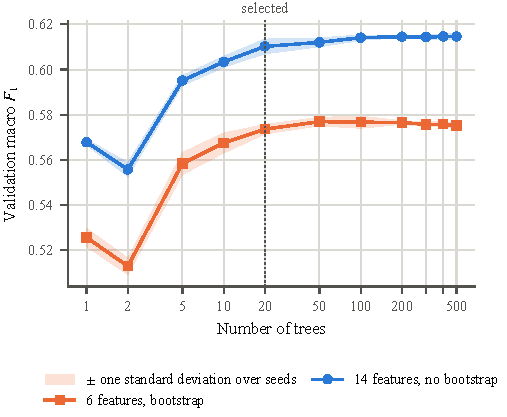
\includegraphics[width=\columnwidth]{trees_final.pdf}
  \caption{Validation macro-averaged $F_1$ score against the number of trees}
  \label{fig:trees}
\end{figure}

\subsection{Sources of randomness}
\label{subsec:res_randomness}
% Data: src/results/sweep_2/scores.csv.
% - Features per split: peak at 14 to 21 (no bootstrap 0.6125 at 14, 0.6159
%   at 21), selected 14. Hypothesis of an intermediate optimum supported in
%   shape, but the optimum sits far above the square-root default (6).
% - At 6 features with the bootstrap the forest (0.5736) is below the single
%   tuned tree (0.5860): the default setting of a random forest is worse
%   than one tree on this data. Strong, quotable point.
% - Bagging (42 features, bootstrap) 0.6085, level with the best bootstrap
%   forest (0.6090 at 21). The hypothesis that bagging is worse is not
%   supported.
% - Why few features per split hurt here: three features (service, sbytes,
%   sttl) carry most of the signal. With 6 of 42 drawn, a split often has
%   none of them, so the trees are weak (high sigma^2) and the lower
%   correlation does not make up for it.
% - Bootstrap: without it the score is higher at every feature count from 1
%   to 21, by 0.007 to 0.011; lower only at 42, where no randomness is left
%   and every tree is the same tree (0.5841, equal to one tree, 0.5853 in the
%   sweep 0 grid for the unlimited tree): a built-in sanity check.
% - Mechanism to offer, as an explanation not a tested claim: the bootstrap
%   hides about 37% of records from each tree, so each tree is weaker; with
%   46.5% duplicates it adds little diversity, because left-out records often
%   have identical copies in the sample. Feature subsampling already gives
%   enough diversity. Cite geurts2006extremely for forests without bootstrap.

Figure~\ref{fig:features} gives the score of the forest against the number
of features per split, with and without the bootstrap. The score rises with
the number of features up to 14 or 21 and falls at 42, so an intermediate
value is best, as the second hypothesis stated. The best
value lies more than twice the usual default, however. Without the bootstrap the
forest scores 0.5841 at six features, 0.6125 at 14 and 0.6159 at 21, and the
one-standard-error rule selects 14. At the default of six features with the
bootstrap, the forest scores 0.5736, below the 0.5860 of the single tuned
tree. The usual setting of a random forest is therefore worse than one tree
on this data.

A possible cause is that the signal is concentrated in a few features. The
service of a flow, the source byte count and the source time to live
carried about two thirds of the importance of the assignment 2 tree. When six of the 42 features are drawn at a split, none of these three is among them
at about 62\% of the splits, against about 29\% when 14 are drawn. Each tree
is then weaker, and the lower correlation between the trees does not make up for it. Section~\ref{subsec:bg_rf} describes the trade-off between the strength of the trees and their correlation.

Section~\ref{subsec:emp_questions} anticipated that bagging, with all 42
features at every split, would score below an intermediate number of
features. Instead, bagging scores 0.6085, level with the best forest with
the bootstrap, at 0.6090 with 21 features. The three shared features therefore
did not lower the score of bagging by a measurable amount.

Dropping the bootstrap raised the score at every number of features from 1
to 21, by between 0.0068 and 0.0105. Only at 42 features did the bootstrap
help, by 0.0244.  That forest scores 0.5841, level with a single tree grown without
limits, as Section~\ref{subsec:bg_rf} predicts.

The bootstrap may cost each tree more than it adds.
Each tree misses about 37\% of the distinct records, which makes it weaker.
The diversity it adds is smaller than usual, because 46.5\% of the records
are duplicates, and a record that the sample missed often has an identical
copy that was drawn. Once the features are subsampled, the trees are
already diverse enough without it. 
%
% [fig] features.pdf: macro F1 and accuracy against features per split, with
% and without the bootstrap (two panels).
\begin{figure}[t]
  \centering
  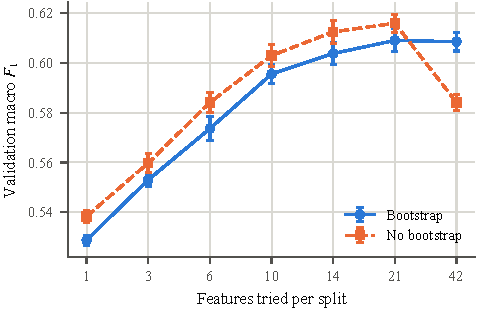
\includegraphics[width=\columnwidth]{features.pdf}
  \caption{Validation macro-averaged $F_1$ score against the number of features per split}
  \label{fig:features}
\end{figure}

\subsection{Tree complexity}
\label{subsec:res_complexity}
% Data: src/results/sweep_0/, sweep_3a/, sweep_3b/ scores.csv.
% - Tree grid (sweep 0): best entropy, depth 30, leaf 5 (0.5883); selected
%   entropy, depth 25, leaf 5 (0.5860, fewest leaves within one standard
%   error). Unweighted. Gini and entropy within noise of each other.
% - Forest depth (3a): rises to 0.6102 at 25, flat to unlimited (0.6125);
%   selected 25. Leaf (3b): falls steadily from 0.6102 at 1 to 0.5415 at 50;
%   selected 1.
% - Hypothesis partly supported: both select depth 25, so the forest does
%   not need deeper trees; but the forest prefers leaf 1 while the tree
%   needs leaf 5. The smaller leaves are the extra complexity averaging
%   tolerates.
% - Overfitting: training macro F1 0.7614 (forest) against 0.6827 (tree);
%   the forest has the larger train-validation difference and the higher
%   validation score, because the variance of its fully grown trees is
%   averaged out.
% - Marker's depth 15: by accuracy the tree grid selects depth 15, leaf 1
%   (0.8215); by macro F1 depth 15 scores 0.5797. The marker's value is the
%   accuracy optimum; carry this into Q5.

The tree grid selects the entropy, a maximum depth of 25 and a minimum leaf
size of 5, without class weights. This tree scores 0.5860, within one standard error of the best tree at
0.5883. The best trees with the Gini index and with class weights also lie
within one standard error, in line with the small differences between the two
impurity measures reported in~\cite{raileanu2004theoretical}.

The left panel of Figure~\ref{fig:complexity} shows that depth beyond 25 neither helps nor harms either model. From depth 25 to unlimited depth, the tree scores
between 0.5850 and 0.5883 and the forest between 0.6100 and 0.6125, and
both are selected at depth 25. Section~\ref{subsec:emp_questions}
anticipated that the forest would tolerate deeper trees than the single
tree. Instead, the single tree is not hurt by depth either, so the two
models select the same depth.

The leaf size separates the two models, as the right panel of Figure~\ref{fig:complexity} shows. The score of the forest falls from
0.6102 with one record per leaf to 0.5970 with two and 0.5415 with 50, and
the rule selects one record per leaf. For the tree the leaf size matters
less, since at depth 25 it scores 0.5826 with one record per leaf and
0.5860 with five. A likely explanation is the weight that one leaf carries.
A leaf of one record follows the noise in the training records closely. In a single tree such a leaf decides
the class of every record that reaches it, while in the forest it is one
vote among twenty.

The forest also fits its training records more closely than the tree. Its
training score is 0.7614 against 0.6827 for the tree, which leaves a difference of
0.1512 from its validation score, against 0.0967 for the tree. The forest has
both the larger difference and the higher validation score, because averaging
removes part of the variance of its fully grown trees without removing
their fit to the training records.
%
\begin{figure}[t]
  \centering
  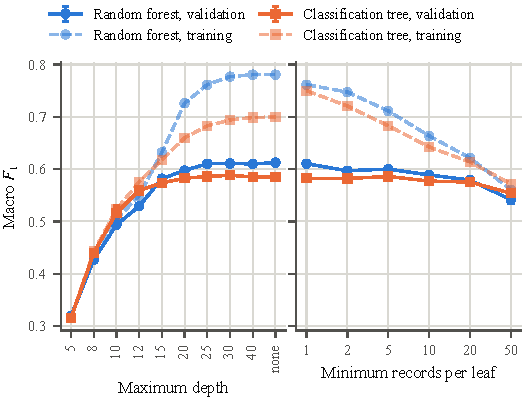
\includegraphics[width=\columnwidth]{complexity.pdf}
  \caption{Training and validation macro-averaged $F_1$ score against maximum depth and minimum leaf size}
  \label{fig:complexity}
\end{figure}

\subsection{Imbalance treatment}
\label{subsec:res_imbalance}
% Data: src/results/sweep_4/scores.csv and treatments.csv. The rare-class
% columns are unweighted means over Worms, Shellcode, Backdoor and Analysis
% (RARE in figures.py); define this in the text before quoting them.
% - No treatment raised macro F1. None 0.6102; SMOTE 5,000 0.6051 (within
%   one standard error); SMOTE 20,000 0.5985; class weights 0.5880; balanced
%   bootstrap 0.4825 (139 per class) rising to 0.5735 (5,000); SMOTE + Tomek
%   0.5711 and 0.5613.
% - Hypothesis part 1 supported: weighting and balancing raise rare-class
%   recall (0.36 to 0.43-0.65) and lower precision (0.69 to 0.11-0.35).
%   Precision falls faster than recall rises, so F1 falls.
% - Balanced bootstrap: score rises with the per-class size because the
%   trees are starved of data (465 leaves at 139 per class, 11,700 without
%   treatment).
% - Hypothesis part 2 supported: Tomek removal lowers F1 for DoS (0.316 to
%   0.169), Backdoor (0.157 to 0.101), Analysis (0.195 to 0.102) against
%   SMOTE alone. Removal at fold 0: 41,312 records, 10,801 of 13,083 DoS.
%   Training macro F1 rises to 0.98 while validation falls: the training
%   set is cleaned of conflicts the validation fold still holds.
% - Backdoor recall rises to 0.614 under SMOTE + Tomek while DoS recall
%   falls to 0.095: with the DoS copies of the conflict groups removed, the
%   tree assigns those regions to Backdoor. Good mechanism paragraph.
% - Caveat: treatments with a swept setting (sizes, targets) had more
%   chances to score well than class weighting.
% - The marker suggested SMOTE with Tomek links; it lowered the score here.
%   Report that plainly with the mechanism; a negative result is a result.

No treatment of the imbalance raised the macro-averaged $F_1$ score above
the 0.6102 of the forest without one, as shown in Table~\ref{tab:treatments}.
SMOTE to 5,000 records per class comes closest, at 0.6051, which is within one
standard error. SMOTE to 20,000 follows at 0.5985, and class weighting at
0.5880. The balanced bootstrap scores lowest, from 0.4825 with 139 records
per class to 0.5735 with 5,000. SMOTE with Tomek links scores 0.5711 and
0.5613 at the two targets. The rule therefore selects no treatment. The
balanced bootstrap and SMOTE each had several settings to choose from,
against one for class weighting, which favoured them, and they still fell
short.

The rare classes below are the four smallest, Worms, Shellcode, Backdoor
and Analysis, and their scores are the unweighted means over the four.
Class weighting and the balanced bootstrap raise the recall of the rare
classes from 0.36 without treatment to between 0.43 and 0.65, and lower
their precision from 0.69 to between 0.11 and 0.35, which is the
pattern the fourth hypothesis described. Precision falls faster than
recall rises, so the $F_1$ score of the rare classes falls, from 0.41 to
between 0.18 and 0.36. The treatments move records of the common classes
into the rare classes, and the common classes are large enough that a small
share of them outnumbers the rare records gained.

The balanced bootstrap improves as the number of records per class rises.
With 139 records per class, each tree is grown on 1,390 records and ends
with about 466 leaves, against about 11,700 without a treatment, so each tree sees too few records
to learn the common classes.

As the fourth hypothesis stated, the removal of Tomek links lowers the score
of Backdoor, DoS and Analysis. Table~\ref{tab:tomek} compares SMOTE alone with SMOTE and Tomek links at 5,000 records per class. Against SMOTE alone, the $F_1$ score falls from 0.316 to 0.169 for DoS, from 0.157 to
0.101 for Backdoor, and from 0.195 to 0.102 for Analysis. The removal took out 41,312 records in the first fold, as reported in Section~\ref{subsec:impl_resampling}. On the cleaned training records the
forest scores 0.9792, while its validation score falls. The removal clears
the conflicting groups from the training records, but the validation
records still hold them, as described in Section~\ref{subsec:bg_imbalance}. The forest therefore learns a problem that is easier than the one it is tested on.

The removal also changes how the forest divides records between DoS and
Backdoor. The recall of
Backdoor rises from 0.108 under SMOTE alone to 0.614, while its precision
falls to 0.055, and the recall of DoS falls from 0.276 to 0.095. The way the
removal empties the conflicting groups may explain this outcome. It leaves
no real records where the groups lay, while the synthetic Backdoor records added by SMOTE, which have
no identical copies, remain nearby. The forest then assigns those regions,
and the many DoS records in them, to Backdoor. 
%
\begin{table}[t]
  \centering
  \caption{Macro-averaged $F_1$ score of each imbalance treatment, with mean scores over the four rarest classes}
  \label{tab:treatments}
  \begin{tabular}{lcccc}
    \toprule
    & & \multicolumn{3}{c}{Rare classes} \\
    \cmidrule(l){3-5}
    Treatment & Macro $F_1$ & Recall & Precision & $F_1$ \\
    \midrule
    \inputtable{../src/results/tables/treatments.tex}
    \bottomrule
  \end{tabular}
\end{table}
\begin{table}[t]
  \centering
  \caption{Per-class scores under SMOTE and SMOTE with Tomek links, at 5,000 records per class}
  \label{tab:tomek}
  \begin{tabular}{llccc}
    \toprule
    Class & Treatment & Precision & Recall & $F_1$ \\
    \midrule
    Backdoor & SMOTE   & 0.287 & 0.108 & 0.157 \\
             & + Tomek & 0.055 & 0.614 & 0.101 \\
    DoS      & SMOTE   & 0.369 & 0.276 & 0.316 \\
             & + Tomek & 0.723 & 0.095 & 0.169 \\
    Analysis & SMOTE   & 0.542 & 0.119 & 0.195 \\
             & + Tomek & 0.063 & 0.287 & 0.102 \\
    \bottomrule
  \end{tabular}
\end{table}

\subsection{Choice of performance measure}
\label{subsec:res_measure}
% Data: src/results/final/measure_choice.csv.
% - The measures disagree in three of six sweeps: tree grid (macro F1:
%   depth 25 leaf 5; accuracy: depth 15 leaf 1), number of trees (20 against
%   100), forest depth (25 against 20). They agree on features and
%   bootstrap, leaf size and treatment.
% - Pattern: accuracy prefers shallower trees and more trees. Mechanism:
%   accuracy is dominated by Normal, Generic and Exploits, which are learnt
%   early; the extra depth that macro F1 rewards serves the rare classes.
% - Answer to the marker's depth comment: 15 is right for accuracy, 25 for
%   macro F1, and the report's primary measure is macro F1.
% - Short subsection: a table of the six pairs may be clearer than prose.

Selecting on accuracy instead of on the macro-averaged $F_1$ score changes
the selection in three of the six sweeps, as shown in Table~\ref{tab:measure}. The two
measures agree on the features per split and the bootstrap, on the leaf
size of the forest and on the imbalance treatment. They disagree on the other three. For the tree grid,
accuracy selects depth 15 with one record per leaf, where the
macro-averaged $F_1$ score selects depth 25 with five. Accuracy also
selects 100 trees rather than 20, and a forest depth of 20 rather than 25.

Where the measures disagree on depth, accuracy prefers the shallower trees,
and the per-class scores in Table~\ref{tab:measure_classes} show which
classes lose by the choice. In the
forest, the shallower trees lower the $F_1$ score of Analysis from 0.204 to
0.115 and that of DoS from 0.329 to 0.297. Only Exploits gains, from 0.722
to 0.732. The tree loses on the same two classes, with
Analysis falling from 0.170 to 0.088 and DoS from 0.318 to 0.277, while
Exploits rises from 0.707 to 0.731. Accuracy rises by at most 0.0049,
because Exploits holds 17\% of the records and Analysis and DoS together
about 7\%. A possible cause is that Analysis and DoS are separated from
Exploits only by the last few splits of a deep tree. A shallower tree
leaves those regions to Exploits, the larger class. Accuracy counts
records, so it rewards the shallower trees, while the macro-averaged $F_1$ score
counts classes, so it does not.

The disagreement on the number of trees has a different cause. The
standard error of accuracy over the folds is about 0.001, against about
0.004 for the macro-averaged $F_1$ score, so the one-standard-error rule
leaves accuracy a narrower margin around its best value, at 300 trees.
Accuracy selects 100 trees, while the macro-averaged $F_1$ score
accepts 20. The choice of measure therefore decides the depth of both
models, and which of the conflicting classes they serve.

\begin{table}[t]
  \centering
  \caption{Configurations selected by each performance measure}
  \label{tab:measure}
  \begin{tabular}{llll}
    \toprule
    Sweep & Parameter & Macro $F_1$ & Accuracy \\
    \midrule
    0  & Tree grid & Depth 25, leaf 5 & Depth 15, leaf 1 \\
    1  & Trees & 20 & 100 \\
    2  & Features, bootstrap & 14, none & 14, none \\
    3a & Maximum depth & 25 & 20 \\
    3b & Minimum leaf size & 1 & 1 \\
    4  & Treatment & None & None \\
    \bottomrule
  \end{tabular}
\end{table}

\begin{table}[t]
  \centering
  \caption{$F_1$ score of three classes under the selection made by each measure}
  \label{tab:measure_classes}
  \begin{tabular}{lcccc}
    \toprule
    & \multicolumn{2}{c}{Tree} & \multicolumn{2}{c}{Forest} \\
    \cmidrule(lr){2-3} \cmidrule(l){4-5}
    Class & Macro $F_1$ & Accuracy & Macro $F_1$ & Accuracy \\
    \midrule
    Analysis & 0.170 & 0.088 & 0.204 & 0.115 \\
    DoS      & 0.318 & 0.277 & 0.329 & 0.297 \\
    Exploits & 0.707 & 0.731 & 0.722 & 0.732 \\
    \bottomrule
  \end{tabular}
\end{table}

\subsection{Comparison with the assignment 2 models}
\label{subsec:res_comparison}
% Data: src/results/final/overall.csv, folds.csv, tests.json, per_class.csv,
% summary.json; LaTeX bodies in src/results/tables/.

\subsubsection{Overall performance}

\begin{table}[t]
  \centering
  \setlength{\tabcolsep}{4pt}
  \caption{Mean performance over the five folds, with the standard deviation in brackets}
  \label{tab:overall}
  \begin{tabular}{lccc}
    \toprule
    Measure & k-NN & Tree & Forest \\
    \midrule
    \inputtable{../src/results/tables/overall.tex}
    \bottomrule
  \end{tabular}
  \\[2pt]
  \parbox{\columnwidth}{\footnotesize The forest scores are means over five
  seeds. Across the seeds, its macro-averaged $F_1$ score has a standard
  deviation of 0.0032, from 0.6069 to 0.6139.}
\end{table}
% [tab] per-fold macro F1 (folds.tex: fold, k-NN, tree, forest).
\begin{table}[t]
  \centering
  \caption{Macro-averaged $F_1$ score per fold}
  \label{tab:folds}
  \begin{tabular}{cccc}
    \toprule
    Fold & k-NN & Tree & Forest \\
    \midrule
    \inputtable{../src/results/tables/folds.tex}
    \bottomrule
  \end{tabular}
\end{table}
\begin{table}[t]
  \centering
  \setlength{\tabcolsep}{4pt}
  \caption{Paired $t$-tests on the macro-averaged $F_1$ score over the five folds, with Holm-adjusted $p$-values}
  \label{tab:tests}
  \begin{tabular}{lcccc}
    \toprule
    Comparison & Difference & 95\% interval & $t$ & $p$ \\
    \midrule
    Forest $-$ tree & 0.0243 & 0.0194 to 0.0291 & 13.93 & 0.00015 \\
    Forest $-$ k-NN & 0.1093 & 0.0954 to 0.1231 & 21.92 & 0.00005 \\
    \bottomrule
  \end{tabular}
\end{table}

The forest reaches the highest score of the three models on every performance
measure.
Table~\ref{tab:overall} reports a macro-averaged $F_1$ score of 0.6102 for the forest,
against 0.5860 for the tree and 0.5010 for the k-nearest neighbours classifier. The same order 
holds for accuracy, where the forest reaches 0.8315 against 0.8166 for the
tree and 0.7717 for the k-nearest neighbours classifier. 

The gain over both models is larger than the variation between folds. The
forest scores higher than the tree and the k-nearest neighbours classifier on each of the five
folds, as shown in Table~\ref{tab:folds}. Table~\ref{tab:tests} reports a paired $t$-test, which puts the mean difference at 0.0243 between the forest and the tree, and at
0.1093 between the forest and the k-nearest neighbours classifier, with
Holm-adjusted $p$-values~\cite{holm1979simple} of 0.00015 and 0.00005.
The forest is
therefore the strongest of the three models on this data.

The size of the gain is more visible when considering the highest score that a
model can achieve. The conflicting duplicate groups limit the maximum
achievable accuracy to 0.9139, as described in Section~\ref{subsec:impl_data}. The accuracy of the tree is 0.0973 below this bound and that of the forest
0.0824 below it, so the forest reduces the difference from the bound by
about 15\%. Nor is the gain the result of a favourable seed: across the five seeds, the
macro-averaged $F_1$ score of the forest has a standard deviation of 0.0032 against a gain of 0.0243 over the tree, as shown in Table~\ref{tab:overall}. The forest therefore
improves on the tree by a margin that holds on every fold, but it remains 0.0824 below the best attainable accuracy.

\subsubsection{Performance per class}
% - The forest is above the tree in every class; largest gains Shellcode
%   (+0.069), Fuzzers (+0.042), Analysis (+0.035), Worms (+0.030).
% - The planned analysis found no link between gain and conflict rate
%   (Spearman rho = -0.02, p = 0.96). State the expectation (gains where
%   conflict is low) and that it was not supported.
% - Conflicting classes stay low: Analysis 0.204, DoS 0.329, Backdoor 0.177.
%   The confusion matrix shows where they go: predicted as Exploits 0.51,
%   0.66, 0.56. Records with identical features cannot be separated by any
%   classifier, so this is a property of the data, not of the model.
% - k-NN is above both tree models for DoS only (0.371 against 0.329).
% - Analysis precision 0.896 with recall 0.116: the forest predicts Analysis
%   rarely but correctly.
%
% [fig] per_class.pdf: F1 per class for the three models, classes ordered
% by conflict rate.
% [fig] confusion_forest.pdf (confusion_tree.pdf if space; probably not).

The forest scores higher than the tree in every one of the ten classes, as shown in Table~\ref{tab:per_class}. Although a class
with many conflicting records leaves less room for any model to improve, the
gains do not follow the conflict rate. The largest gains are in Shellcode (0.069),
Fuzzers (0.042), Analysis (0.035) and Worms (0.030), classes with conflict
rates from 0.9\% to 77.0\%, and the rank correlation between the gain and the
conflict rate is close to zero (Spearman $\rho = -0.02$, $p = 0.96$). 

The three classes with the most conflicting records remain the weakest for
every model. Analysis, DoS and Backdoor have conflict rates of 77.0\%, 77.4\%
and 84.9\%, and the forest reaches $F_1$ scores of only 0.204, 0.329 and 0.177
on them. Table~\ref{tab:per_class} also shows where their records go, since
the forest predicts 51\% of Analysis, 66\% of DoS and 56\% of Backdoor records as
Exploits. Records with identical features cannot be separated by any
classifier, which makes these errors a property of the data rather than of
the model. The forest also predicts Analysis rarely but accurately, with a precision of 0.896 against a recall of 0.116.

DoS is the one class on which the k-nearest neighbours classifier scores
higher than both tree models,
with an $F_1$ score of 0.371 against 0.329 for the forest and 0.318 for the
tree.
% [tab] per_class.tex: class, conflict %, k-NN, tree, forest F1.
\begin{table}[t]
  \centering
  \setlength{\tabcolsep}{4pt}
  \caption{Conflict rate, $F_1$ score per class, and share of each class that the forest predicts as Exploits}
  \label{tab:per_class}
  \begin{tabular}{lccccc}
    \toprule
    & & \multicolumn{3}{c}{$F_1$ score} & Forest to \\
    \cmidrule(lr){3-5}
    Class & Conflict (\%) & k-NN & Tree & Forest & Exploits (\%) \\
    \midrule
    \inputtable{../src/results/tables/per_class.tex}
    \bottomrule
  \end{tabular}
\end{table}

\subsubsection{Feature importance}
% - The top three features (service, sbytes, sttl) hold 68% of the tree's
%   importance and 38% of the forest's; 90% is reached with 10 features in
%   the tree and 22 in the forest. Features per split force other features
%   into the trees.
% - The ten features removed from the k-NN pipeline hold 9.8% (tree) and
%   15.4% (forest): their removal in assignment 2 cost little.
% - Caveat: impurity importance favours features with many distinct values
%   (cite strobl2007bias).
% - Data: src/results/final/importances.csv, summary.json; figure
%   importance.pdf if space.

The forest spreads its importance over more features than the tree, as shown in Table~\ref{tab:importance}. The
three leading features, the service of a flow, the source byte count and
the source time to live, account for 0.68 of the importance of the tree but
0.38 of that of the forest. The tree needs 10 features to reach 0.90 of its
importance, and the forest needs 22. The service of a flow falls from 0.30
of the importance in the tree to 0.13 in the forest, and the source time to
live from 0.18 to 0.09.

The spread follows from the features drawn at each split. With 14 of the
42 features drawn, none of the three leading features is available at about
29\% of the splits, as found in Section~\ref{subsec:res_randomness}. At those splits the tree must split on another feature. Features that the single tree barely used then
gain importance. The number of connections with the same destination
address and source port rises from 0.002 of the importance in the tree to
0.055 in the forest, and the number of connections in each state for a
range of time to live values rises from 0.001 to 0.042. The second of these
is built from the time to live, so it may stand in for the source time to
live when that feature is not drawn.

The ten features removed from the k-nearest neighbours classifier in
assignment 2 account for 0.10 of the importance of the tree and 0.15 of
that of the forest. Their removal therefore discarded little of the
information that the trees use. These shares carry the bias of
impurity-based importance described in Section~\ref{subsec:bg_tree}.


\begin{table}[t]
  \centering
  \caption{Feature importance of the tree and the forest}
  \label{tab:importance}
  \begin{tabular}{lcc}
    \toprule
    Feature or summary & Tree & Forest \\
    \midrule
    Service of a flow                  & 0.30  & 0.13  \\
    Source byte count                  & 0.19  & 0.16  \\
    Source time to live                & 0.18  & 0.09  \\
    Same destination and source port   & 0.002 & 0.055 \\
    Connections per state and TTL      & 0.001 & 0.042 \\
    \midrule
    Share of the top three             & 0.68  & 0.38  \\
    Features to reach 0.90             & 10    & 22    \\
    Share of the ten removed for k-NN  & 0.10  & 0.15  \\
    \bottomrule
  \end{tabular}
\end{table}

\subsubsection{Computational cost}
% - Fold 0, lab machine, 8 cores: fit 3.7 s (tree), 7.1 s (20-tree forest);
%   prediction 13.8 million rows/s (tree), 2.6 million (forest), 2,111
%   (k-NN, one thread, assignment 2). Say the threads differ.
% - The 500-tree forest took about 170 s per fit; the 20-tree selection
%   costs about 4% of that.
% - Source: src/results/final/timing.json, summary.json.

The forest takes about twice as long as the tree to fit, and both classify
records more than a hundred times faster than the k-nearest neighbours classifier. Table~\ref{tab:cost} reports the costs on the first fold. The tree took 3.7 seconds to fit and the 20-tree forest 7.1 seconds.
The forest grows twenty trees in about twice the time of one, because its
trees are built in parallel on eight cores and each of its splits searches
14 features in place of 42. A forest of 500 trees, which Section~\ref{subsec:res_trees} found to score about 0.0045 higher, took about 170 seconds to
fit, so the selected forest costs about 4\% of that.

The forest classified 2.6 million records per second, against 13.8 million
for the tree and 2,111 for the k-nearest neighbours classifier. Even with a perfect use of eight threads in place of its one, the classifier
would remain more than a hundred times slower than the forest. The difference follows from how each model
classifies. A tree follows one path of at most 25 tests, and the forest
follows one such path in each of its 20 trees, while the k-nearest
neighbours classifier measures the distance to every one of about 206,000
training records, as described in Section~\ref{subsec:bg_knn}. 

\begin{table}[t]
  \centering
  \caption{Fit time and prediction rate on the first fold}
  \label{tab:cost}
  \begin{tabular}{lcc}
    \toprule
    Model & Fit (s) & Records per second \\
    \midrule
    k-NN (one thread) & --  & 2,111 \\
    Tree              & 3.7 & 13.8 million \\
    Forest, 20 trees  & 7.1 & 2.6 million \\
    Forest, 500 trees & 170 & -- \\
    \bottomrule
  \end{tabular}
\end{table}

\subsection{Limitations}
\label{subsec:res_limitations}
% - Own subsection (style guide section 7). Each limitation as a mechanism,
%   with a number.
% - Tuning and evaluation share the folds: optimistic bias.
% - One question at a time: interactions between parameters are not
%   searched (the tree count is the one checked).
% - Paired t-test on dependent folds.
% - k-NN not retuned; it was tuned on a subsample in assignment 2 and
%   selected k = 1 with Manhattan distance, an edge value of its grid.
% - Treatments with swept settings had more chances.
% - Simplified nominal distance in SMOTE.
% - Impurity importance bias.
% - Results are for one synthetic dataset.

As described in Section~\ref{subsec:emp_cv}, the same five folds were used to tune the models and to evaluate them, so the reported scores are biased upwards
and are not estimates on unseen records. The tree was selected from 240
configurations and the forest from 52, so the tree had more chances to fit
the folds, and the bias is unlikely to explain the higher score of the forest.

The parameters were tuned one at a time, so their interactions were only
partly searched. The number of trees was checked again for the final
configuration, and lies 0.0045 below the score of 500 trees, as reported in Section~\ref{subsec:res_trees}. The depth and the leaf size were not
checked in the same way, and both were selected with 20 trees.

The paired $t$-tests treat the five fold differences as independent,
although any two training folds share three quarters of their records, so
their $p$-values are too small, as noted in Section~\ref{subsec:bg_stats}. The forest scores higher than both models on all five folds, so the conclusion does not rest on the
$p$-values alone.

The k-nearest neighbours classifier was not tuned again. In assignment 2 it
was tuned on a stratified subsample of 40,000 records, where one neighbour
led three by 0.0002, well inside the noise. Tuning on the full training folds might change its score, but a change as
large as its deficit of 0.1093 is unlikely. A class weighting of its vote,
which would favour the rare classes, has no effect at one neighbour, because
a single vote cannot be outweighed. It would need a larger $k$, and the
classifier scored lower at every larger $k$ in assignment 2.

As described in Section~\ref{subsec:impl_resampling}, the SMOTE distance gives each nominal mismatch the weight of one standard deviation, a simplification of the SMOTE paper. A different weight would
change which records are neighbours, and therefore both the synthetic
records and the Tomek links found.

The importances are based on the decrease in impurity, which favours
features with many distinct values, as described in Section~\ref{subsec:bg_tree}. The
service of a flow and the source time to live have only 13 distinct values
each, against up to 121,356 for other features, so the bias does not
explain their high importance. The importance of the features with many values, such
as the source byte count with 9,382, is likely to be overstated.

The results hold for one dataset, whose attacks were generated
synthetically and whose ordinary traffic was recorded in one laboratory, as described in Section~\ref{subsec:bg_dataset}. The share of duplicated records, 46.5\%,
drives two of the findings, the weak bootstrap and the failure of the
removal of Tomek links, and may be lower in traffic recorded elsewhere.

% =============================================================================
\section{Conclusion}
\label{sec:conclusion}
% Worth 4. One or two paragraphs.
% - Restate the headline with its number (0.6102 against 0.5860 and 0.5010).
% - One sentence per research question, naming which expectations were wrong:
%   bagging was not worse; the bootstrap hurt; depth was not deeper.
% - The limit set by the data: the conflicting classes.
% - Next steps as short numbered sentences ("The first is..."): a separate
%   test split or nested cross-validation; joint tuning of trees and
%   features; deduplication or label resolution of the conflicting groups;
%   probability averaging in place of the majority vote.

A random forest was tuned and evaluated on the UNSW-NB15 dataset and
compared with the classification tree and the k-nearest neighbours
classifier of assignment 2. The selected forest of 20 trees, with 14
features per split, no bootstrap and trees of depth 25, scores 0.6102 on
the macro-averaged $F_1$ score, against 0.5860 for the tree and 0.5010 for
the k-nearest neighbours classifier, and scores higher than both on every fold.
Its score levels off after a few tens of trees. Although bagging was
expected to score worse, it scored level with the best forest that uses the
bootstrap, and dropping the bootstrap raised the score at every number of
features below 42. The forest needed the same depth as the tree and gained
instead from leaves of one record. None of the imbalance treatments
improved on using no treatment, and SMOTE with Tomek links lowered the
score of the three classes with the most conflicting records. Selecting on
accuracy chose shallower trees, at the cost of Analysis and DoS.

 The forest reduces the difference between the accuracy of the tree and the
best attainable accuracy of 0.9139 by about 15\%. Analysis, DoS and
Backdoor, most of whose records sit in conflicting duplicate groups, remain
the weakest classes for every model, and their errors are a property of the
data rather than of the model.

Four steps would extend this work. The first is to evaluate the selected
models on records held out from tuning, by a separate test split or by
nested cross-validation. The second is to tune the number of trees together
with the features per split and the bootstrap. The third is to resolve the
conflicting duplicate groups and measure how much of the remaining error
they explain. The fourth is to replace the majority vote by the average of
the class proportions in the leaves, which breaks ties by the confidence of
the trees.

% =============================================================================
\bibliographystyle{IEEEtranS}
\bibliography{references}
% Worth 4. Only cited entries appear in the list.

\end{document}
